\documentclass[12pt,a4paper,oneside]{ctexart}
\usepackage{amsmath,amsthm,amssymb,wrapfig,graphicx,float,tabularx}
\title{切变模量实验报告}
\author{张博厚 PB22071354}
\date{2023.6.12}
\begin{document}
\maketitle
\tableofcontents
\newpage
\section{实验背景与目的}
切变模量,又称剪切模量/刚性模量,材料的力学性能指标之一,是指材料在剪切应力作用下,
在弹性变形比例极限范围内,切应力与切应变的比值.切变模量表征材料抵抗切应变的能力,模量大,则表示材料的刚性强.本实验中
采用扭摆实验装置来测量金属丝的切变模量,尽量避免测量较难测准的物理量,提高实验精度.
\section{实验原理}
本实验的实验对象是一根上下均匀而细长的钢丝,在几何上可认为是一个半径为
$R$,长度为$L$的细长圆柱体.将钢丝上端固定,下端面发生扭转,则在弹性限度内有
\begin{equation}
    \tau = G\gamma
\end{equation}
式中$G$即为材料的切变模量,如下图所示:
\begin{figure}[H]
    \centering
    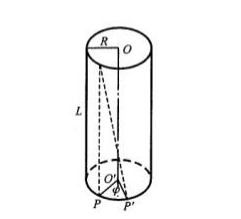
\includegraphics[scale=1.2]{扭转形变示意图.png}
    \caption{金属丝扭转形变示意图}
\end{figure}
设钢丝下端面绕中轴线转过的角度为$\phi$(图中P点转到P'点),根据位错理论,
金属丝各截面均相应地发生了转动,其单位长度的转角$\frac{d\phi}{dl}=\frac{\phi}{L}$,
选取其中长为$dl$的体积元,可以推知在其中半径为$\rho$的位置,切应变为
\begin{equation}
    \gamma_{\rho}=\rho\dfrac{d\phi}{dl}
\end{equation}
其产生的恢复力矩
\begin{equation}
    dM=\tau_{\rho}\cdot\rho\cdot2\pi\rho\cdot d\rho=2\pi G\rho^3\dfrac{d\phi}{dl}\cdot d\rho
\end{equation}
故总力矩为
\begin{equation}
    M=\int_0^R2\pi G\rho^3\dfrac{d\phi}{dl}\cdot d\rho=\dfrac{\pi}{2}GR^4\dfrac{d\phi}{dl}=\dfrac{\pi}{2}GR^4\dfrac{\phi}{L}
\end{equation}
为求出钢丝的恢复力矩,在其下端悬挂一圆盘,可绕中轴线自由扭动,则摆扭过的角度正比于所受的扭力矩:
\begin{equation}
    M=D\phi
\end{equation}
又由转动定律,
\begin{equation}
    M=I_0\dfrac{d^2\phi}{dt^2}
\end{equation}
联立(5)(6),得
\begin{equation}
    \dfrac{d^2\phi}{dt^2}+\dfrac{D}{I_0}\phi=0
\end{equation}
这是一个简谐运动微分方程,其周期为
\begin{equation}
    T_0=2\pi\sqrt{\dfrac{I_0}{D}}
\end{equation}
但作为扭摆的圆盘上有一个夹具,并不对称,直接计算$I_0$比较困难,因此可将
一个金属环对称地置于圆盘上.设环的质量为$m$,内外半径分别为$r_1,r_2$,易知其转动惯量为
$I_1=\frac{1}{2}m(r_1^2+r_2^2)$,则此时扭摆周期为
\begin{equation}
    T_1=2\pi\sqrt{\dfrac{I_0+I_1}{D}}
\end{equation}
联立(4)(5)(6)(8)(9),得
\begin{equation}
    D=\dfrac{2\pi^2m(r_1^2+r_2^2)}{T_1^2-T_0^2}
\end{equation}
\begin{equation}
    G=\dfrac{4\pi Lm(r_1^2+r_2^2)}{R^4(T_1^2-T_0^2)}
\end{equation}
\section{实验内容}
\subsection{实验仪器}
扭摆装置,螺旋测微器,游标卡尺,米尺,秒表
\subsection{实验步骤}\noindent
1. 调整扭摆装置,使钢丝与圆盘面垂直,圆环能方便地置于圆盘上.\\
2. 用螺旋测微器测量钢丝直径,用游标卡尺测量环的内外径,用米尺测量钢丝的有效长度.\\
3. 写出相对误差公式,据此估算应测量的周期数目.\\
4. 选定扭转角度,测量放置金属环前后多个周期的时长.\\
5. 计算钢丝的切变模量 G 和扭转模量 D,完成误差分析.\\
6. 测量不同扭转角度下的周期,研究钢丝的切变模量与其扭转角度的关系.
\subsection{方案设计}
在实验中,直接测量量为金属丝,金属环的直径,将式(11)改写为
\begin{equation}
    G=\dfrac{16\pi Lm(d_1^2+d_2^2)}{d^4(T_1^2-T_0^2)}
\end{equation}
根据最大不确定度公式,有
$$\dfrac{\Delta G}{G}=\dfrac{\Delta L}{L}+\dfrac{\Delta m}{m}
        +\dfrac{2d_1\Delta d_1}{d_1^2+d_2^2}+\dfrac{2d_2\Delta d_2}{d_1^2+d_2^2}
        +4\dfrac{\Delta d}{d}+\dfrac{2T_0\Delta t_0}{N_0(T_1^2-T_0^2)}+\dfrac{2T_1\Delta T_1}{N_1(T_1^2-T_0^2)}$$
其中$N_0,N_1$分别为待测周期数,粗侧数据如下:

\section{数据记录与处理}
\section{思考与讨论}
\end{document}